\subsection{Self-supervised Class-priors Estimation}
\label{sec:pi_estim}
Instead of fixing the values of $\bm{\pi}$ before training as in~\cite{kiryo17}, we instead propose to refine all values iteratively during training. Our approach, which we refer to as Self-Supervised Non-Negative PU Learning (\SSnnPU), will start with a large-upper bound for $\pi_i$ and will progressively reduce the estimates at each epoch of our training scheme until a stopping criterion is reached. That is, we will optimize the function $f_\theta$ one epoch at a time using Alg.~\ref{alg:sgdnnpu}, and the use the intermediary model to help estimate the class priors.

However, deriving class prior estimates from partial models (\ie trained with few epochs) yields very noisy estimates with large variances. Hence, we propose to use a Bayesian framework to estimate the class priors in a recursive fashion by establishing a state space and observation model and inferring the class priors. We now describe our approach in more detail by first formalizing the state and observation models, and we describe our recursive Bayesian estimate and stopping conditions thereafter. Our final training algorithm is summarized in Alg.~\ref{alg:prior_estim}.

\subsubsection{State and Observation models}
Recall $\bm{\pi}_k=\{\pi_{k}^{i}\}_{i=1}^N$ to be the true class prior of a sequence of $N$ frames. While we wish to know $\bm{\pi}$, our method 
will compute values $\bm{\hat\pi}=\{\hat\pi^{i}\}_{i=1}^N$ as the best approximation to $\bm\pi$. At the same time, our prediction model after $k$ training epochs, denoted $f_{\theta_k}$, can also provide partial information to the value of $\bm\pi$. Specifically, by evaluating $f_{\theta_k}$ on all samples $x \in \mathcal{X}^i$, we can estimate a noisy observation of $\pi^i$ by computing the expected value over $f_{\theta_k}$,
\begin{equation}
  \label{eq:observ}
\rho_{k}^{i} = \mathbb{E}_{x \in \mathcal{X}^{i}}[f_{\theta_{k}}(x)^{\gamma}].
\end{equation}
\noindent 
Here, $\gamma > 1$ is a correction factor that mitigates variations in the expectation at different epoch values. That is, we wish that our prediction model slightly over-segment the object of interest so to over-estimate the frequencies of positives. This is because we wish to progressively decrease $\bm{\hat\pi}$ from its initial value $\hat \pi_{0}$ by using $\bm{\rho}_{k}$ as observations. 

To do this, we denote $\bm{\pi_k} $ and $\bm{\hat\pi_k}$ to be true and inferred class priors after epoch $k$. While the value $\bm{\pi_k} $ is the same for all values of $k$, we include this notation at this stage to define the following linear state observation model we will use to infer $\bm{\hat\pi_k}$,
\begin{align}
\bm{\bm{\pi}}_{k+1} &= g(\bm{\pi}_{k}, L) - u_{k}\mathbf{1}_{N} + \mathcal{N}(0,Q),\label{eq:trans_fn}
\end{align}
\noindent
where $\bm{\bm{\rho}}_{k} \sim \mathcal{N}(\bm{\pi}_{k},R)$,
$\bm{\pi}_{0}  \sim \mathcal{N}(\hat\pi_{0},S)$, and $Q$, $R$, and $S$ are the transition, observation, and initial covariance matrices, respectively. The function $g(\cdot, L)$ is a moving average filter of length $L$ with a Hanning window to impose a frame-wise smoothness. For convenience, we write $\mathbf{1}_{N}$ for a vector of length $N$ taking values of $1$, and the term $u_{k}$ is the control input,
\begin{equation}
u_{k} = u_{0} + (u_{T} - u_{0})\frac{k}{T},
\end{equation}
\noindent
where $u_{0}$ and $u_{T}$ are two scalars such that $u_{T} > u_{0}$.
The control input therefore induces a downward acceleration on the states and imposes a ``sweeping'' effect on the latter, which allows in principle the range $[0; \hat \pi_{0}]$ to be explored. Last, we also set $\forall i, \hat \pi^i_0 = \pi_{max} >> \pi^{i} $.

%\begin{align}
%\bm{\bm{\tilde\pi}}_{k+1} &= g(\bm{\tilde\pi}_{k}, L) - u_{k}\mathbf{1}_{N} + \mathcal{N}(0,Q), \quad \tilde\pi_{k}^{i} \in [0; \pi_{{max}}] \label{eq:trans_fn}\\
%\bm{\bm{\rho}}_{k} &= \bm{\tilde\pi}_{k} + \mathcal{N}(0,R) \label{eq:proc_fn} \\
%\bm{\tilde\pi}_{0}&=\hat \pi_{0} + \mathcal{N}(0,S) \label{eq:init_fn}
%\end{align}

%\subsubsection{Observation model}
%\label{sec:obs_model}
%We are now interested in inferring robust obervations from our prediction model.
%For clarity, we write $f_{\theta_{k}}$ for our prediction model trained for $k$ epochs.
%Let $f_{\theta_{k}}(x)$ the prediction given by $f_{\theta_{k}}$ on superpixel $x$ at iteration $k$.
%We therefore compute $\rho_{k}^{i}$, the observation at time $k$ on frame $i$ as:
%
%\begin{equation}
%  \label{eq:observ}
%\rho_{k}^{i} = \mathbb{E}_{x \in \mathcal{X}^{i}}[f_{\theta_{k}}(x)^{\gamma}]
%\end{equation}
%
%With $\gamma > 1$ a correction factor.
%This correction is justified as follows: As early iterations use class-priors that are above the true values,
%our prediction model tends to over-segment the object of interest and therefore over-estimate the frequencies of positives.

\begin{algorithm}[t]
\caption{Self-supervised Non-Negative PU Learning}
\label{alg:prior_estim}
\begin{algorithmic}[1]
\Require{$\hat \pi_{0}$: Upper-bound on class-priors \newline
  $T$: Number of epochs \newline
  $f_\theta$: Foreground prediction model}
\Ensure {Optimal estimate of class-prior $\bm{\hat{\pi}}^{*}$\newline}
\State $k = 0$
\State $ {\hat{\pi}^i}_{0} = \pi_{max}, \forall i$
\While {Stopping condition not satisfied}
    \State Optimize $f_\theta$ for $1$ epoch using Alg.~\ref{alg:sgdnnpu} and $\bm{\hat{\pi}}_{k}$
	%\STATE Forward pass all images to get $\bm{y}_k$
    \State Compute observations $\bm{\rho}_k$ as in Eq.~\eqref{eq:observ}
    \State Clip $\bm{\rho}_{k}$ to $[0,\hat \pi_{0}]$
    %\STATE Denote $\bm{\hat\Pi}_{k-1}$ the sigma-points of $\bm{\hat\pi}_{k-1}$
    %\STATE Clip $\bm{\hat\Pi}_{k}$ to $[0, \hat \pi_{0}]$
    %\STATE Transform $\bm{\hat\Pi}$ through the state-transition function to get $\bm{\hat\Pi}_{k+1}^{-}$
    %\STATE Clip $\bm{\hat\Pi}_{k+1}^{-}$ to $[0, \hat \pi_{0}]$
    \State Compute $\bm{\hat\pi}_{k+1}$ using UKF with $\bm{\rho}_{k}$ and $\bm{\hat\pi}_{k}$
    \State	 $k \gets k+1$
\EndWhile
\end{algorithmic}
\end{algorithm}

\subsubsection{Recursive Bayesian Estimation}
Given our linear model Eq.~\eqref{eq:trans_fn}, we wish to compute an optimal estimate of $\bm\pi$ by the conditional expectation,
\begin{equation}
  \label{eq:cond_mean}
\bm{\hat\pi}_{k} = \mathbb{E}[\bm{\pi}_{k} | \bm{\rho}_{0:k}],
\end{equation}
\noindent
where $\bm{\hat\pi}_k$ is the optimal estimate of $\bm{\pi}_{k}$ given the sequence of observations $\bm{\rho}_{0}$ to $\bm{\rho}_{k}$, which we denote $\bm{\rho}_{0:k}$. Note that, Eq.~\eqref{eq:cond_mean} requires one to compute the posterior probability density function (PDF) $p(\bm{\pi}_{k}|\bm{\rho}_{0:k})$, 
\begin{equation}
  \label{eq:aposteriori}
  p(\bm{\pi}_{k}|\bm{\rho}_{0:k}) = \frac{p(\bm{\pi}_{k}|\bm{\rho}_{0:k-1})\cdot p(\bm{\rho}_{k}|\bm{\pi}_{k})}{p(\bm{\rho}_{k}|\bm{\rho}_{0:k-1})},
\end{equation}
\noindent where,
\begin{equation}
  \label{eq:prior}
  p(\bm{\pi}_{k}|\bm{\rho}_{0:k-1}) = \int p(\bm{\pi}_{k}|\bm{\pi}_{k-1}) \cdot p(\bm{\pi}_{k-1}|\bm{\rho}_{0:k-1}) d\bm{\pi}_{k-1},
\end{equation}
\noindent
is a recursive expression of the state at time $k$ as a function of time $k-1$ and the most recent observations.
%The bottom term of Eq. \ref{eq:aposteriori} is a normalization factor that writes:

%\begin{equation}
%  \label{eq:norm_cst}
%  p(\bm{\rho}_{k}|\bm{\rho}_{0:k-1}) = \int p(\bm{\pi}_{k}|\bm{\rho}_{0:k-1}) \cdot p(\bm{\rho}_{k}|\bm{\pi}_{k}) d\bm{\tilde\pi}_{k}
%\end{equation}

%Our state-space model provides expressions of the state-transition probability $p(\bm{\tilde\pi}_{k}|\bm{\tilde\pi}_{k-1})$ via Eq. \ref{eq:trans_fn}, and likelihood $p(\bm{\rho}_{k}|\bm{\tilde\pi}_{k})$ via Eq. \ref{eq:proc_fn}.

Typically, one distinguishes two phases during recursive Bayesian filtering: prediction and correction phase. In the prediction phase, we compute the a-priori state density (Eq. \ref{eq:prior}) using the transition function (Eq. \ref{eq:trans_fn}).
In the correction phase, a new observation vector is available to compute the likelihood $p(\bm{\rho}_{k}|\bm{\tilde\pi}_{k})$ and normalization constant, whereby allowing the a-posteriori state estimate to be computed using Eq.~\eqref{eq:aposteriori}.

Modeling the states as a multi-variate gaussian random variable with additive gaussian noise greatly simplifies this computation, especially when assuming that the transition and observation models are linear. In particular, the latter assumptions typically allows for Kalman Filter type solutions~\cite{kalman1960}. However, the present scenario imposes an inequality constraint on the states so as to make them interpretable as probabilities, a requirement that standard Kalman Filters does not allow for. Instead,~\cite{gupta07} suggests applying an intermediate step in which the a-priori state estimates are projected on the constraint surface. This approach, despite being effective, requires the solving a quadratic program at each iteration.
\begin{figure*}[t]
\caption{Visualization of our SSnnPU method on an example MRI volume. (Top row): Single slice from volume with groundtruth segmentation highlighted (red) and a point-wise annotation (green), output prediction at different epochs. (Bottom row): Class priors at corresponding epochs over 75 slices of the volume. The different curves correspond to: the true priors (blue), observations $\rho_{k}$ (orange), proportion of pseudo-positives (green), and current estimated priors $\hat\pi_{k}$ (red). The stopping condition is triggered at epoch 71.}
\centering
    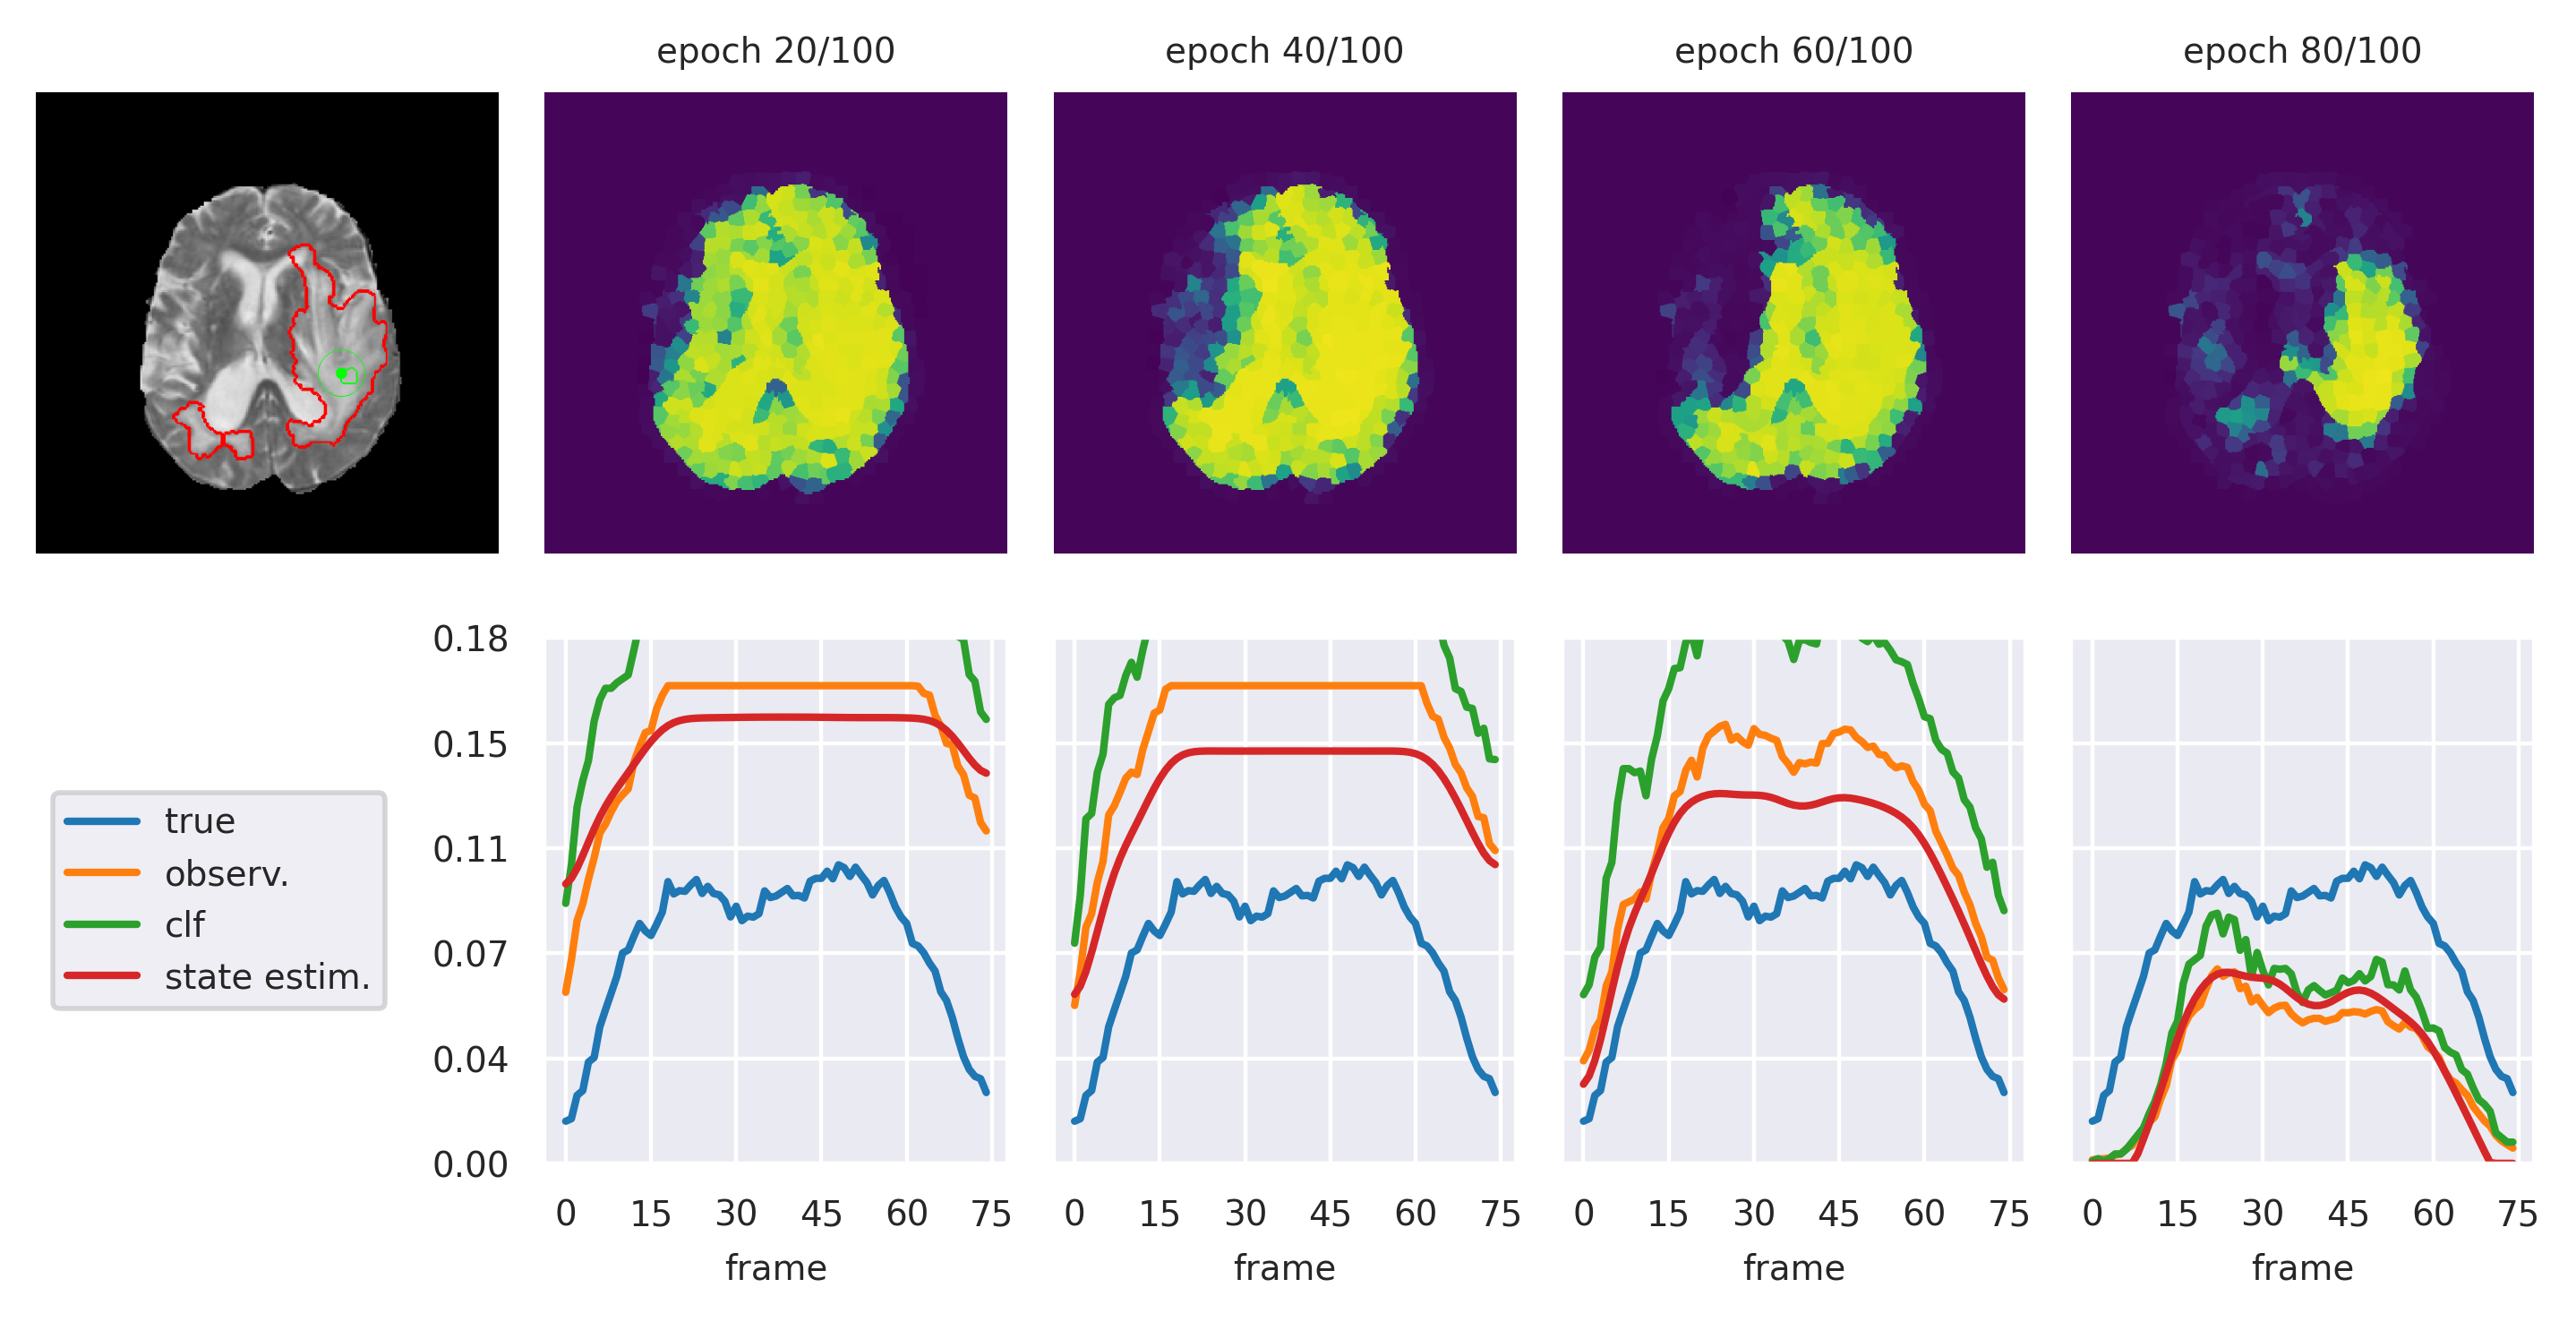
\includegraphics[width=.9\textwidth]{pics/prevs_conv.png}
\label{fig:prevs_conv}
\end{figure*}

Instead, we use the simpler approach of~\cite{kandepu08}, which relies on the Unscented Kalman Filter (UKF) approach~\cite{wan00}. In contrast with standard Kalman Filters, which propagate the means and covariances of states through the (linear) system, UKF samples a set of carefully chosen points from the state distribution, called {\it sigma-points}, that allow to accurately approximate the true statistics of the posterior. Our inequality constraints are then directly applied to the sigma-points.
% TODO: introduce capital pi

As illustrated in Fig.~\ref{fig:prevs_conv}, our self-supervised approach iteratively decreases its estimates of $\pi^i$ (red line) as a function of epoch computed and observations $\rho_{k}^{i}$. Given the defined control inputs $u_k$ which induce a downward acceleration, $\pi^i$ are reduced further than they should be (see epoch 80 in Fig.~\ref{fig:prevs_conv}). For this reason, we introduce a strategy to halt this computation at an appropriate moment in the next section. 

\subsubsection{Stopping condition}
We introduce two stopping conditions that we use simultaneously to ensure that our methods stops at an appropriate value for $\bm\hat\pi$.

Specifically, first we denote $\bm{\tilde{\mathcal{X}}}_{n}=\{x \in \bm{\mathcal{X}} | f_{\theta}(x) < 0.5\}$, and $\bm{\tilde{\mathcal{X}}}_{p}=\{x \in \bm{\mathcal{X}} | f_{\theta}(x) \geq 0.5\}$ as the set of ``pseudo-negative'' and ``pseudo-positive'' samples, respectively.
As a first criteria, we use the variance of the predictions of  $\bm{\tilde{\mathcal{X}}}_{n}$, written $Var[f_{\theta}(\bm{\mathcal{\tilde X}}_{n})]$, which measures the confidence of our model on the negative samples (\ie background regions of the image).
Second, we also impose that our predictions are such that the frequency of positives is below our upper-bound on all frames. By combining these, our criteria (1) imposes a maximum on the frequencies of pseudo-positives, (\ie $\frac{|\bm{\tilde \mathcal{X}}_{p}^{i}|}{N_{i}} < \hat \pi_{0} \quad \forall i$) and (2) imposes a maximum variance level to pseudo-negatives (\ie $Var[f_{\theta}(\bm{\mathcal{\tilde X}}_{n})] < \tau$).

In practice, we want the above conditions to be verified for several iterations so as to guarantee stability. We therefore impose that both conditions are satisfied for $T_{s}$ iterations. In Fig.~\ref{fig:prevs_conv}, we illustrate the behaviour of our stopping conditions by showing the predicted probabilities and their corresponding class-priors on a given sequence.

%In particular, we denote $C(\bm{\hat \pi}_{k})$ a boolean function that represents the above conditions, and select the optimal prior $\bm{\hat \pi}^{*}$ as
%\begin{multline}
%  \label{eq:prior_opt}
%  \bm{\hat \pi}^{*} = \bm{\hat \pi}_{k} \quad \text{iff} \quad C(\bm{\hat \pi}_{k}) \wedge
%  C(\bm{\hat \pi}_{k+1})
%  \wedge \cdots \wedge  C(\bm{\hat \pi}_{k+T_{s}})
%\end{multline}
 


%%% Local Variables:
%%% mode: latex
%%% TeX-master: "main"
%%% End:
